\documentclass{article}[12pt]

% useful packages
\usepackage{titlesec}
\usepackage{fullpage}
\usepackage{amsmath,amssymb,amsthm,amsfonts}
\usepackage{graphicx}
\usepackage{enumerate}
\usepackage{algorithm,algorithmic}
\usepackage{xcolor}
\usepackage{bbm}
\usepackage{url}
\usepackage{hyperref}

% theorem type environments
\newtheorem{thm}{Theorem}
\newtheorem{prop}{Proposition}
\newtheorem{lemma}{Lemma}
\newtheorem{cor}{Corollary}
\newtheorem{defn}{Definition}
\newtheorem{assump}{Assumption}
\newtheorem{example}{Example}
\newtheorem{conjecture}{Conjecture}

% frequently used symbols
\newcommand{\bE}{\mathbb{E}}
\newcommand{\bP}{\mathbb{P}}
\newcommand{\bQ}{\mathbb{Q}}
\newcommand{\bR}{\mathbb{R}}
\newcommand{\bS}{\mathbb{S}}
\newcommand{\bN}{\mathbb{N}}
\newcommand{\bZ}{\mathbb{Z}}
\newcommand{\sC}{{\mathcal C}} 
\newcommand{\sD}{{\mathcal D}} 
\newcommand{\sE}{{\mathcal E}} 
\newcommand{\sF}{{\mathcal F}} 
\newcommand{\sL}{{\mathcal L}} 
\newcommand{\sH}{{\mathcal H}} 
\newcommand{\sN}{{\mathcal N}} 
\newcommand{\sO}{{\mathcal O}} 
\newcommand{\sP}{{\mathcal P}} 
\newcommand{\sR}{{\mathcal R}} 
\newcommand{\sS}{{\mathcal S}}
\newcommand{\sU}{{\mathcal U}} 
\newcommand{\sX}{{\mathcal X}} 
\newcommand{\sY}{{\mathcal Y}} 
\newcommand{\sZ}{{\mathcal Z}}

% operators
\newcommand{\sign}{\mathop{\mathrm{sign}}}
\newcommand{\supp}{\mathop{\mathrm{supp}}} % support
\newcommand{\argmin}{\operatornamewithlimits{arg\ min}}
\newcommand{\argmax}{\operatornamewithlimits{arg\ max}}
\newcommand{\dist}{\operatorname{dist}}
\newcommand{\tr}{\text{tr}}
\newcommand{\vecop}{\text{vec}}
\newcommand{\st}{\operatorname{s.t.}}
\newcommand{\cut}{\setminus}
\newcommand{\ind}[1]{\mathbbm{1}\left\{#1\right\}} 
\newcommand{\given}{\ | \ }

% grouping operators
\newcommand{\brac}[1]{\left[#1\right]}
\newcommand{\set}[1]{\left\{#1\right\}}
\newcommand{\abs}[1]{\left\lvert #1 \right\rvert}
\newcommand{\paren}[1]{\left(#1\right)}
\newcommand{\norm}[1]{\left\|#1\right\|}
\newcommand{\ip}[2]{\left\langle #1,#2 \right\rangle}

% code commands
\newcommand{\matlab}{\textsc{Matlab }}
\newcommand{\python}{\textsc{Python }}
\newcommand{\todo}[1]{\textcolor{red}{#1}}

% header command
\newcommand{\project}[3]{
    \pagestyle{myheadings}
    \thispagestyle{plain}
    \newpage
    \setcounter{page}{1}
    \setlength{\headsep}{10mm}
    \noindent
    \begin{center}
    \framebox{
        \vbox{\vspace{2mm}
            \hbox to 6.28in { {\bf EE 519: Deep Learning Theory \& Fundamentals
            \hfill Spring \the\year} }
        \vspace{4mm}
        \hbox to 6.28in { {\Large \hfill Mini Project #1 \hfill} }
        \vspace{2mm}
        \hbox to 6.28in { \Large \hfill Due: #2, 11:59PM PT \hfill }
        \vspace{2mm}
        \hbox to 6.28in { {\it Student Name: #3} \hfill {\it Instructor Name: John Lipor}}
        \vspace{2mm}}
   }
   \end{center}
   \markboth{Mini Project #1}{Mini Project #1}
   \vspace*{4mm}
}

\begin{document}

% PUT YOUR NAME BELOW WHERE I HAVE \X
\project{1}{April 28, \the\year}{Andy Franck}
% PUT YOUR NAME ABOVE WHERE I HAVE \X

\section*{Problem Description}

\indent
The objective of this project is to develop a neural network model capable of accurately categorizing geothermal heat flow residuals into one of four distinct classes. These residuals will be compared against actual heat flow measurements to assess the suitability of a geothermal energy site at the given location.\\
\indent
To accomplish this, a dataset consisting of 28 features, including heat flow residuals, will be used to train a neural network model. The model will be trained on a subset of the data, and then tested on the remaining data. The model will be evaluated based on its ability to correctly classify the heat flow residuals into one of the four classes.\\ 
\indent
The training data is provided from both the United States Geological Survey \cite{USGS}, and the INGENIOUS project \cite{INGENIOUS}. The data includes feature vectors provided by multiple surveys and sources. The data has been modified into an 80/20 training/validation split, and the validation data is separated from the model until it testing. \\
\indent
Although it would be convenient to have an easy-to-train model that can make accurate predictions, it is not guaranteed that any such model will work properly. This report aims to develop a model that has the highest possible correct classification rate with the given feature vectors and training data. 
Certainly, as our population continues to grow, finding economical sources of energy becomes more and more prudent. Developing a model that can accurately predict locations where a surrogate for geothermal energy is favorable would be an excellent development in our search for more sustainable energy.



\section*{Exploratory Data Analysis}

To establish a baseline for exploratory data analysis (EDA), two articles \cite{EDA1}, \cite{EDA2} were consulted in addition to a video tutorial by Rob Mulla \cite{RobMulla}. The articles provided a general overview of EDA, and the video tutorial provided a more in-depth look at the process.\\
\indent
To gain a preliminary understanding of the correlations of all features/labels, a correlation plot was generated using the Seaborn library. These visualizations helped to identify high correlations between certain features and the labels, as well as between pairs of features.\\

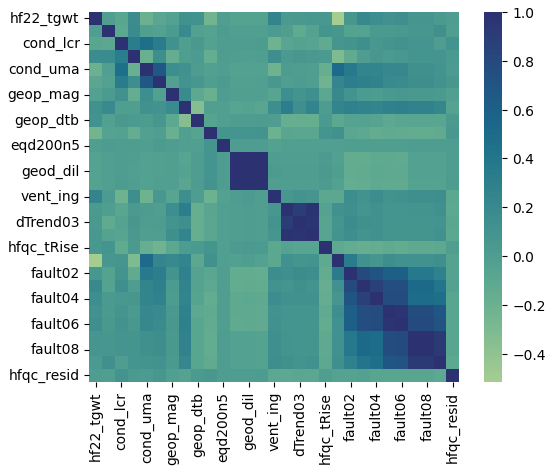
\includegraphics[width=0.5\textwidth]{seaborn-1.png}
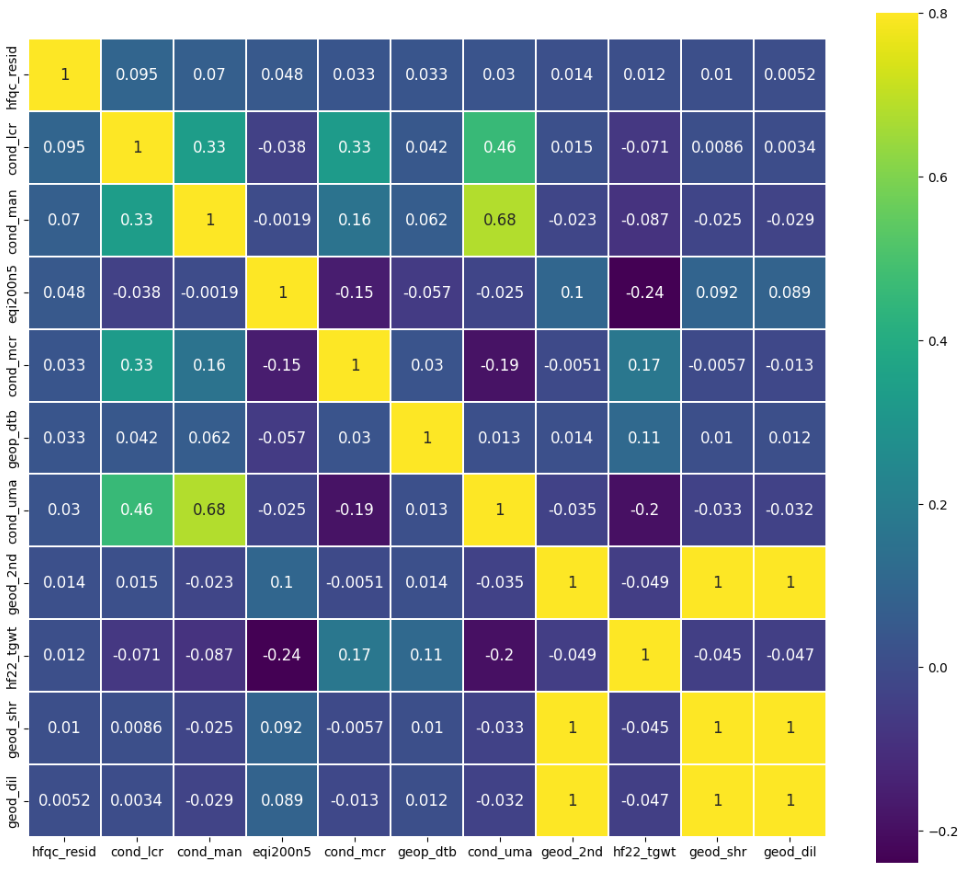
\includegraphics[width=0.5\textwidth]{seaborn-2.png}\\

\indent
It is easy to determine from the images which features have a high correlation to each other. For example, \emph{geop\_dtb} and \emph{cond\_mcr} both have similar features, so it is not necessary to include both. Also notice \emph{cond\_lcr} has an extremely high correlation to the residuals, so it is included as one of the featuers.\\
\indent

To get a more general description of the data, the pandas.describe() function was used. This function provides a summary of the data, including the mean, standard deviation, minimum, maximum, and quartiles.\\

\begin{center}
    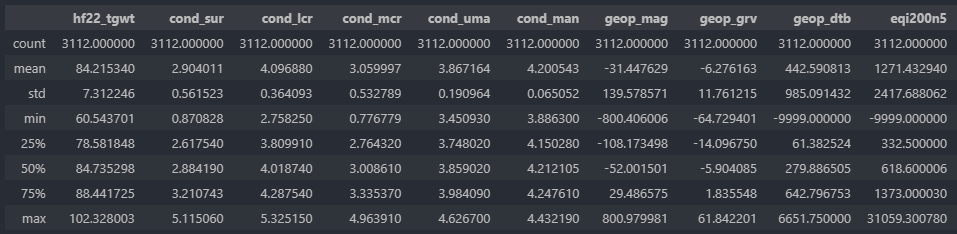
\includegraphics[width=0.9\textwidth]{describe.png}\\
\end{center}

\indent
From this data, it is easy to determine which features contain outliers and empty values. For example, the features \emph{} and \emph{eqi200n5} have minimum values of $-9999$. These outliers need to be removed from the data to assist the model in training. To confirm visually, box and whisker plots were generated for each feature.\\

\begin{center}
    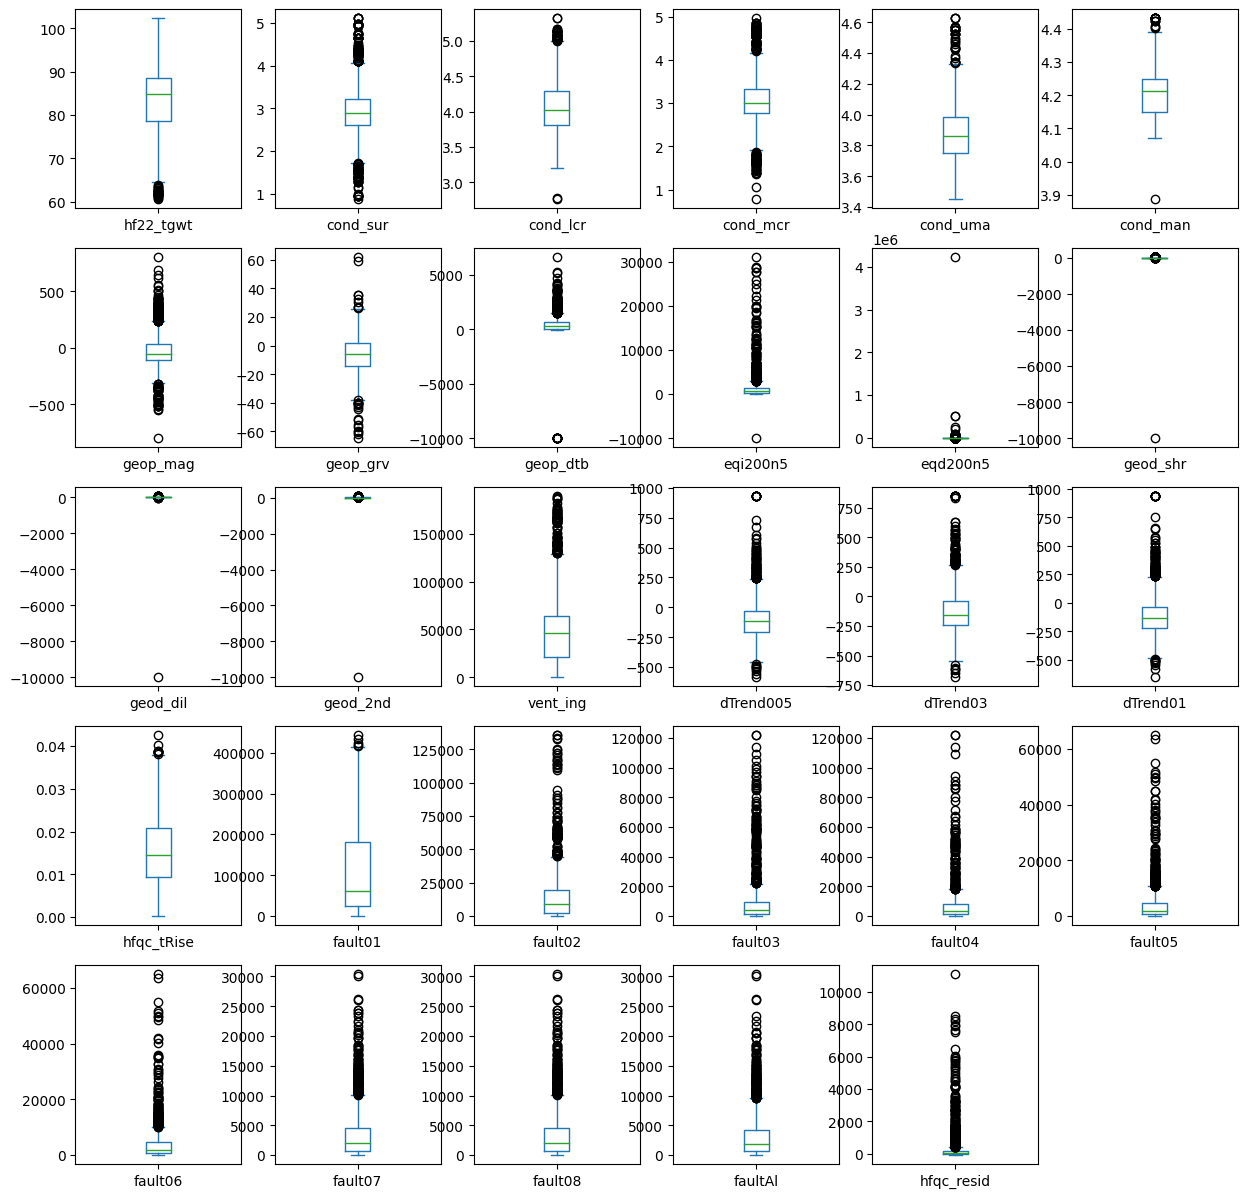
\includegraphics[width=0.6\textwidth]{box-whisker.png}
\end{center}

Finally, histograms were plotted for each feature to assess whether the data was normally distributed. If the data is not normally distributed, it can reduce the accuracy of the model dramatically.\\

\begin{center}
    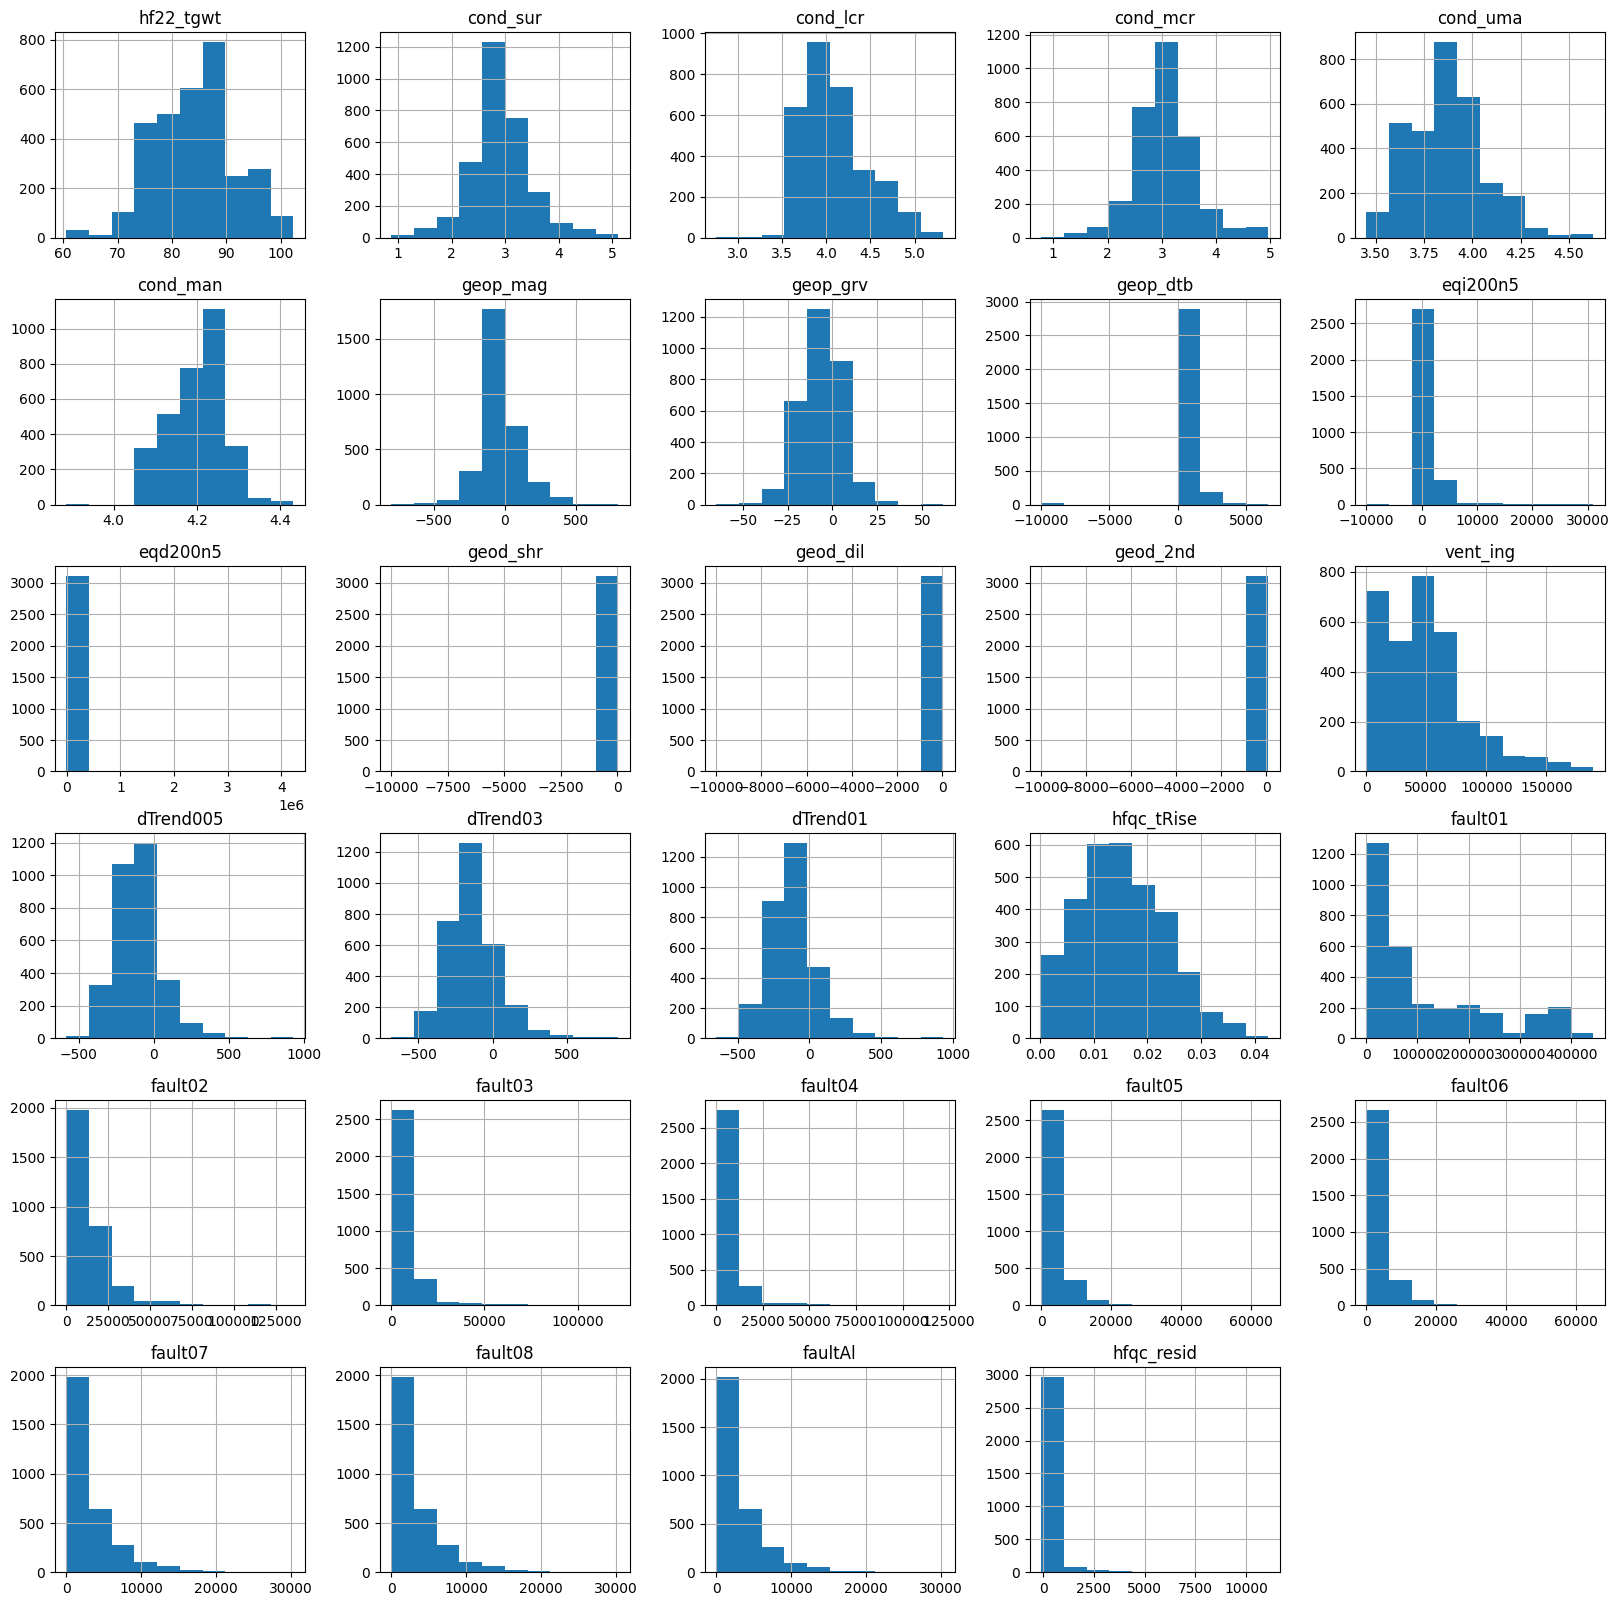
\includegraphics[width=0.6\textwidth]{histogram.png}
\end{center}

To address the non-normality of the data displayed above, a quantile transform was applied to the features. This transform maps the data to a normal distribution.\\

\begin{center}
    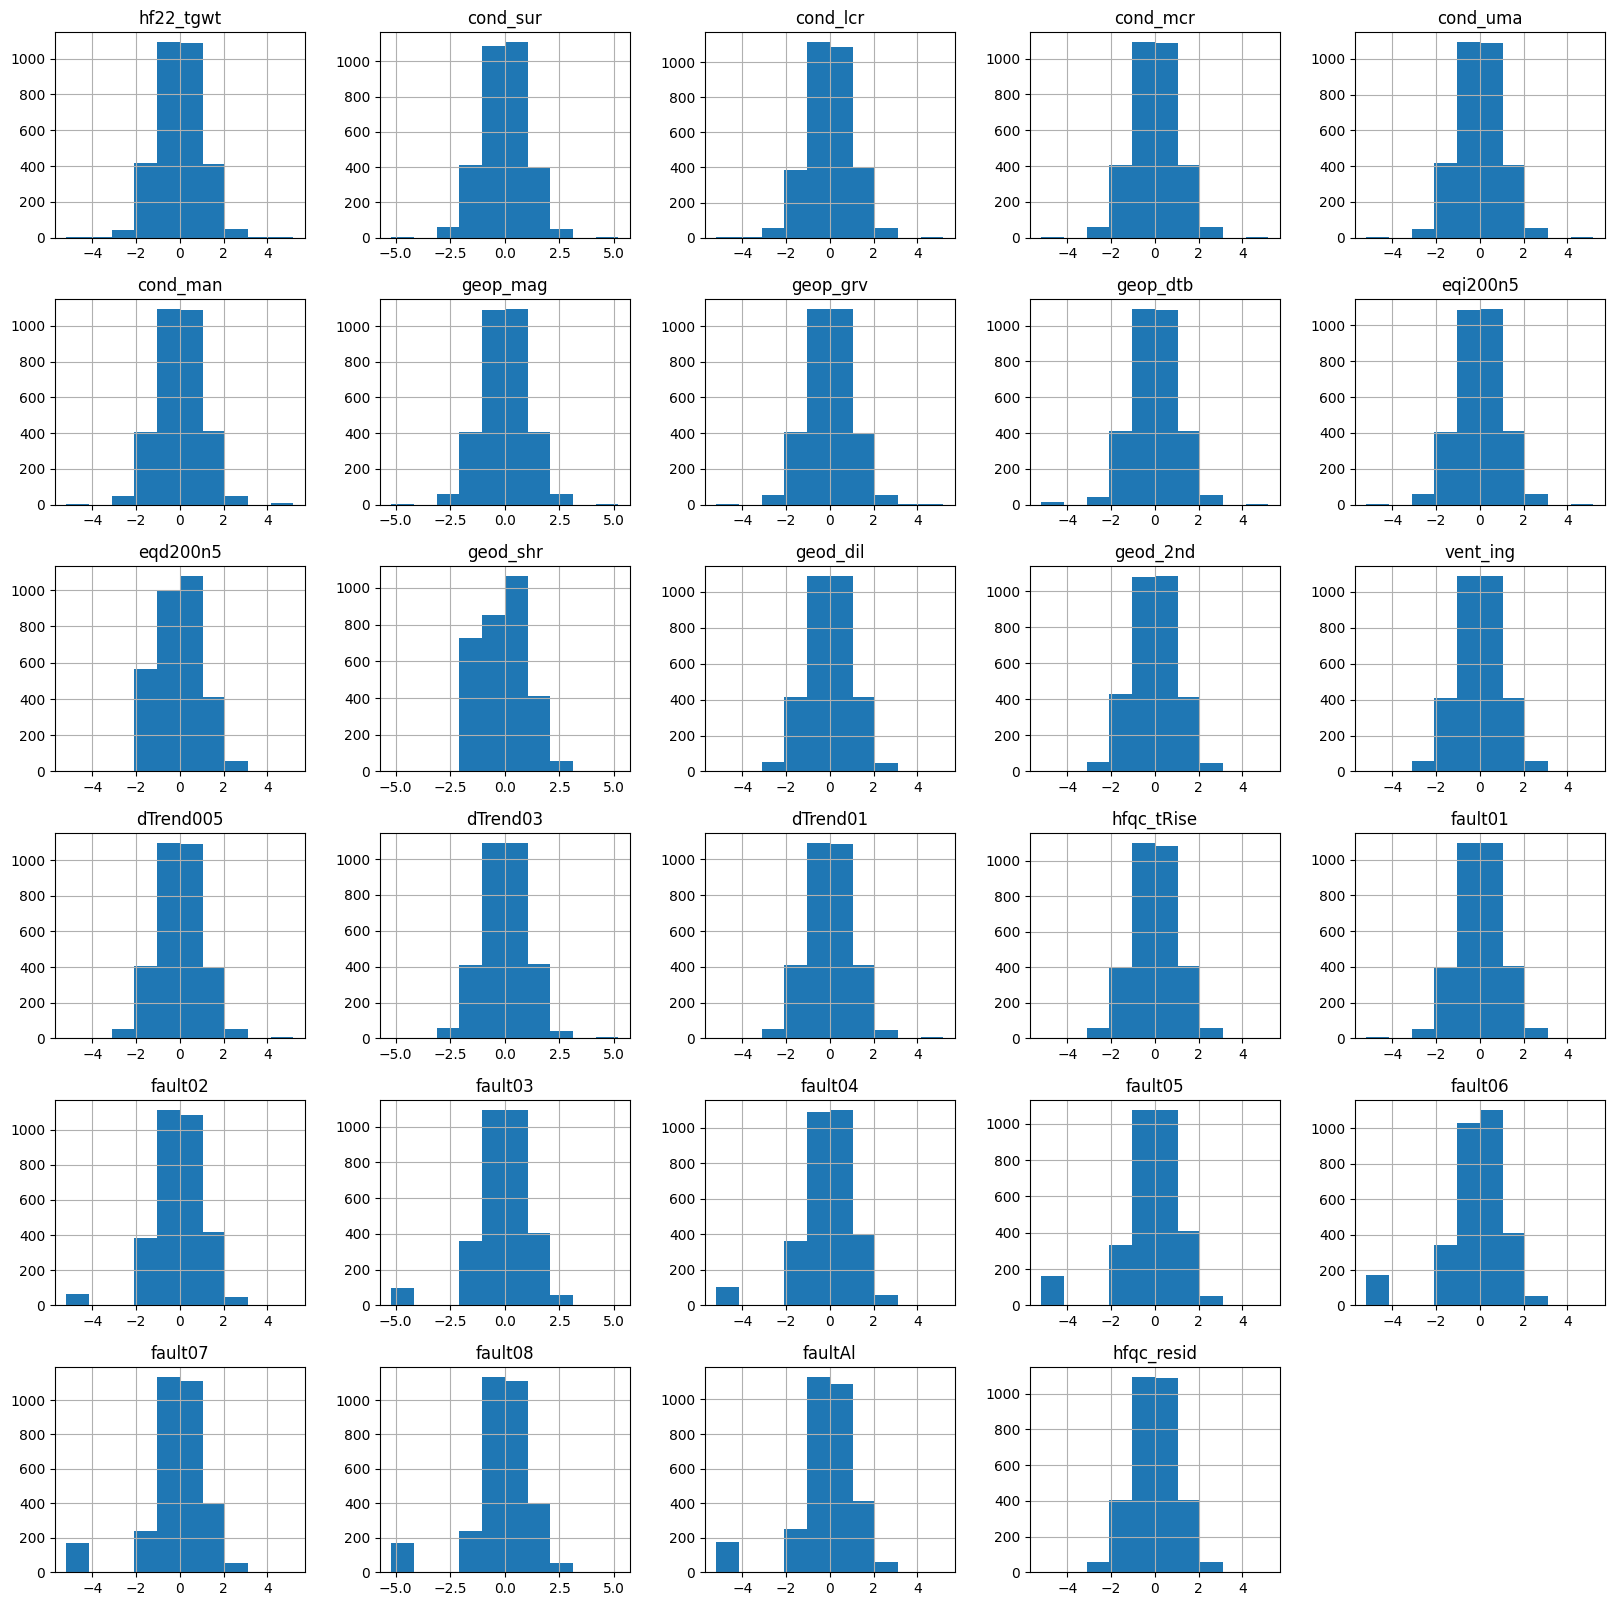
\includegraphics[width=0.6\textwidth]{histogram_after_quantile_with_labels.png}
\end{center}

\section*{Challenges}

The data management phase presented the main challenges of the project. Despite the relative simplicity of the MLP itself, managing the data types and transformations proved to be the most persistent challenge.
\indent
One of the major obstacles was convering the data to types that the different libraries could accept. This required a lot of trial and error to identify the root of the data type issues. Moreover, managing transformations and ensuring they were properly performed and then reverted in the correct order was also a challenge.\\
\indent
The model's accuracy was often significantly impacted by my improper implementaions of the transformations and reversals. Additionally, performing the transformations in combination with the train/validation split was also a challenge. Often, some of the modifictations required a full dataset to be present, so it was necessary to save the original features, attach the output, perform the transformation, then pull out the output and save it separately. This would then be repeated for the validation set, and then reverted in the proper order.\\
\indent
Finally, the d2l library was also a source of significant frustration. Importing the library into Colab often resulted in obscure errors that were not the cause of incorrect code. As a result, the code was modified to use a pure PyTorch implementation instead of the d2l library.\\


\section*{Approach}

The initial step in the development involved creating a simple working model that analyzed a sample of the data. Although the results were not satisfactory, this model provided a baseline for the development of the final model. After the baseline model was created, the model was then updated and trained on all 3112 samples and 16 features, which were chosen from the EDA applications and recommended features provided in the project description. The DataLoader function was used to load the data into the model.\\

\indent
The preprocessing of the data did not require significant data wrangling, as the pandas DataFrame method used to load the data made it very easy to access and move. However, the data did require some transformations to ensure the model could properly train. The data was converted to a PyTorch tensor, and then the data was normalized using the mean and standard deviation of the training data. The application of each preprocessing method was fopllowed by a training and testing of the model for perforamce gain and accuracy, which was measure by Colab's built in timer aned the ratio of correct predictions to total predictions, respectively. By recommendation of \cite{Validation_Medium}, the testing/validation split was 80/20 percent, randomly shuffled. The validation set was kept hidden from the data during the training phase to avoid any bias, and all preprocessing methods were applied to it seperately.\\
\indent
To increase performance and reduce overfitting, PCA was applied to the training and validation\cite{PCA_Medium}. The first 8 principal components were found to account for almost all of the variance in the data, so the remaining components were dropped. However, saving all the principal components was essential to transform the data back to the original space for classifying the validation set.\\

\begin{center}
    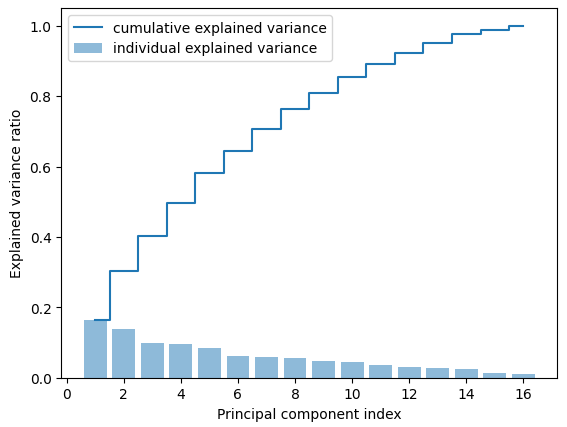
\includegraphics[width=0.4\textwidth]{PCA.png}
\end{center}

\indent
Since the data was also not in normal distribution, a quantile transform was applied to the data to map it to a normal distribution (see EDA section). This was done to increase the accuracy of the model, as non-normal data can reduce the accuracy of the model significantly.\\
\indent
Since outliers were present in the data, they were removed using the IQR method \cite{IQR}. A function was created to remove the outliers from the data. The function calculates the first and third quartiles (Q1 and Q3), as well as the IQR (Q3 - Q1), for each column. It then defines upper and lower thresholds for outliers as 1.5 times the IQR above Q3 and below Q1, respectively. Values outside of these thresholds are replaced with the median value of the column.\\

\begin{center}
    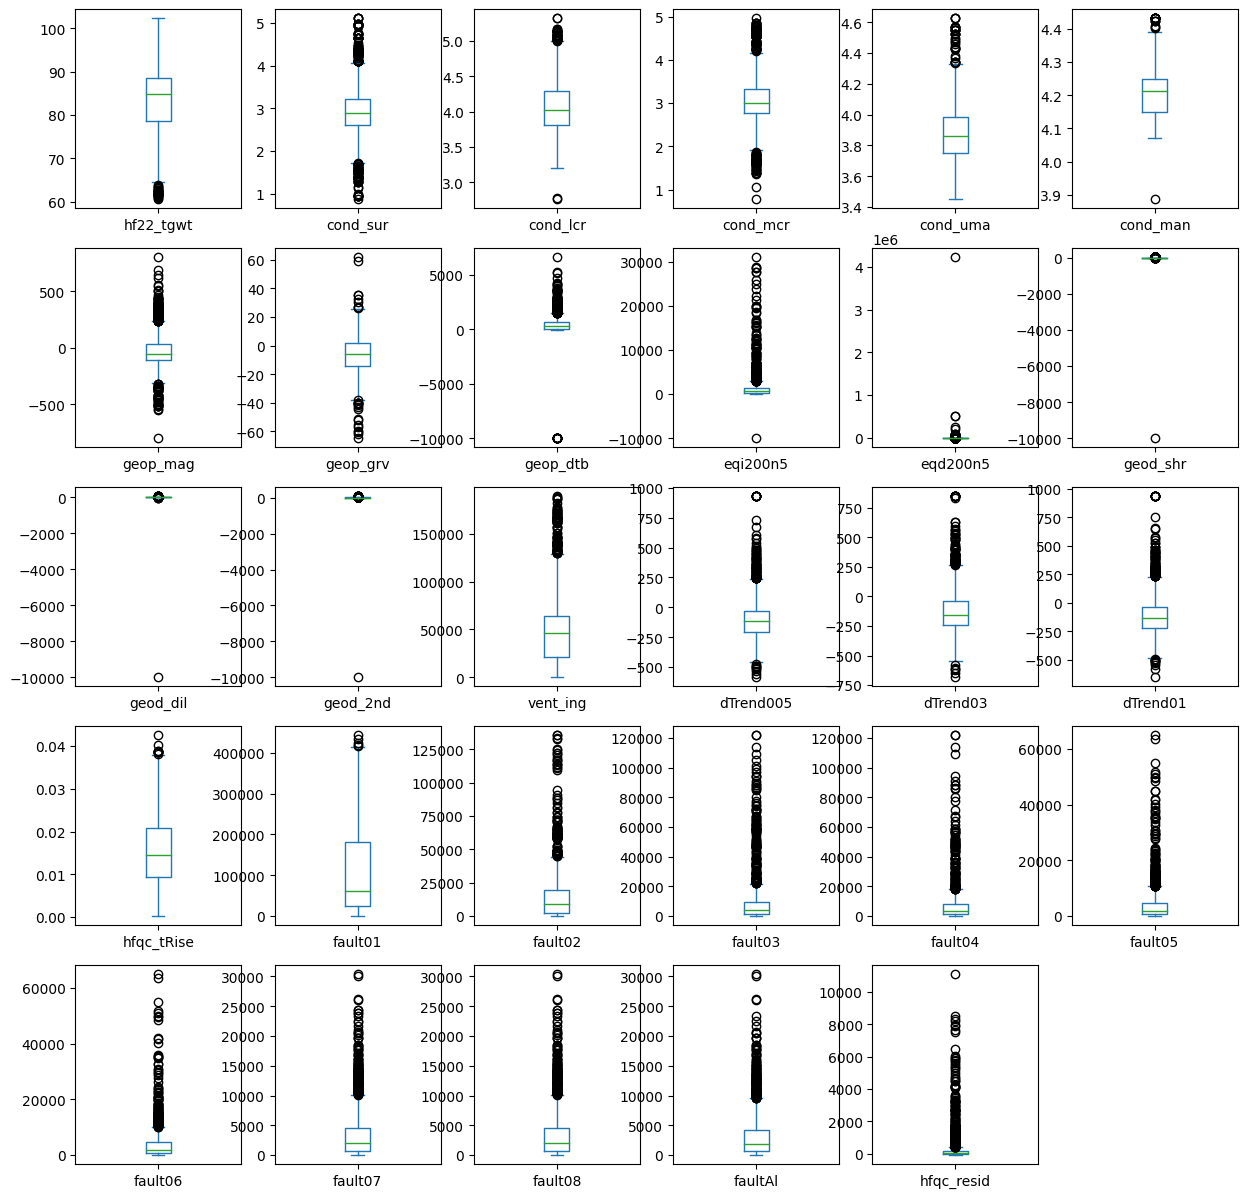
\includegraphics[width=0.6\textwidth]{box-whisker.png}
    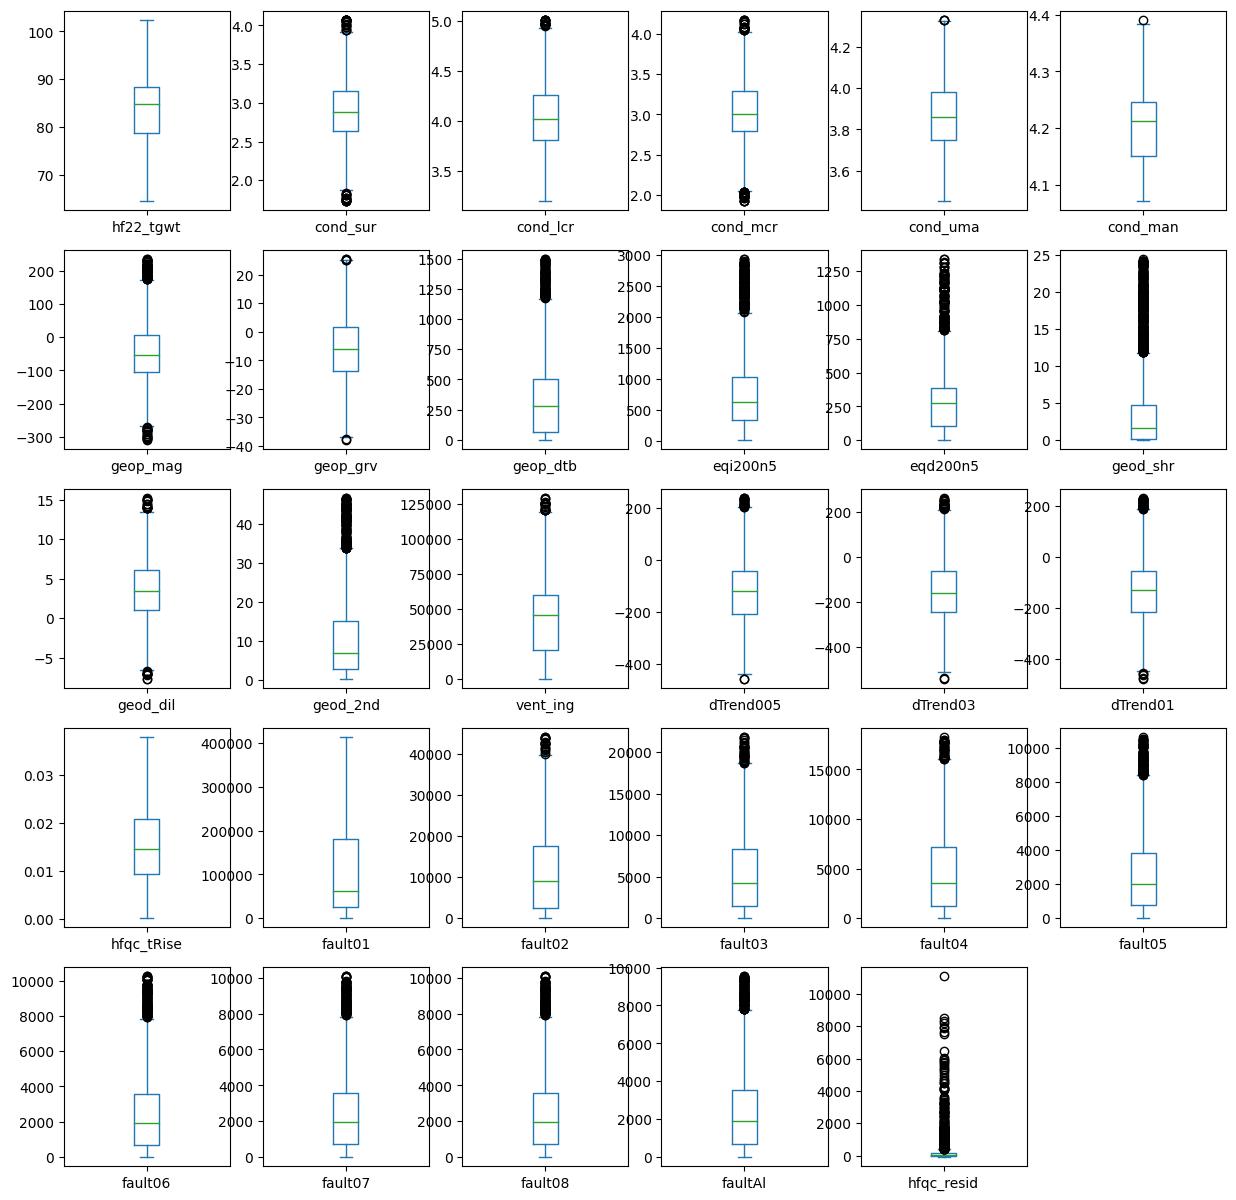
\includegraphics[width=0.6\textwidth]{box-whister-after-outliers.png}
\end{center}

\indent
Because there were so many outliers, it was counterproductive to remove all of them. Instead, the outliers were replaced with the median value of the feature. This was done to avoid losing too much data.\\
\indent
Finally, the data was split into training and validation sets. The training set was used to train the model, and the validation set was used to test the model. The validation set was kept hidden from the model during the training phase to avoid any bias.\\
\indent
The model was then trained using the training set. It was trained for 10,000 epochs, at a batch size of 350. The hyperparameters were suggested based on the recommendations of \cite{Design_NN_Medium}. These suggestions were inputted into Optuna \cite{optuna_2019}, which is a hyperparameter optimization library. Suggestions for multiple different loss functions were intially provided, however Adam consistently outperformed the competition, so it was the clear choice, averaging nearly 10\% higher accuracy averages than the second best alternative.\\


\section*{Evaluation and Summary}

Unfortunately, the trained model did not perform to the level of accuracy desired. The model was able to achieve an average classification accuracy of 52\%. Fortunately, although the model was not particularly accurate, it seemed to be consistent, as the accuracy was very similar for each of the 5 folds.\\
\indent
The model was also able to stay fairly consistent between both validation and test loss. Both values were very similar, although the validation loss was slightly higher. This is likely due to the fact that the validation set was not used to train the model, so it was not as familiar with the data.\\

\begin{center}
    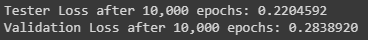
\includegraphics[width=0.3\textwidth]{loss.png}
\end{center}

\indent
The following SHAP graph is a good model of which features positively and negatively impaced classification. For example, the feature \emph{vent\_ing} either had a very positive or very negative impact on the classification. A feature like \emph{dTrend005} appears relatively helpful for classification, while others appear not particularly useful at all.\\

\begin{center}
    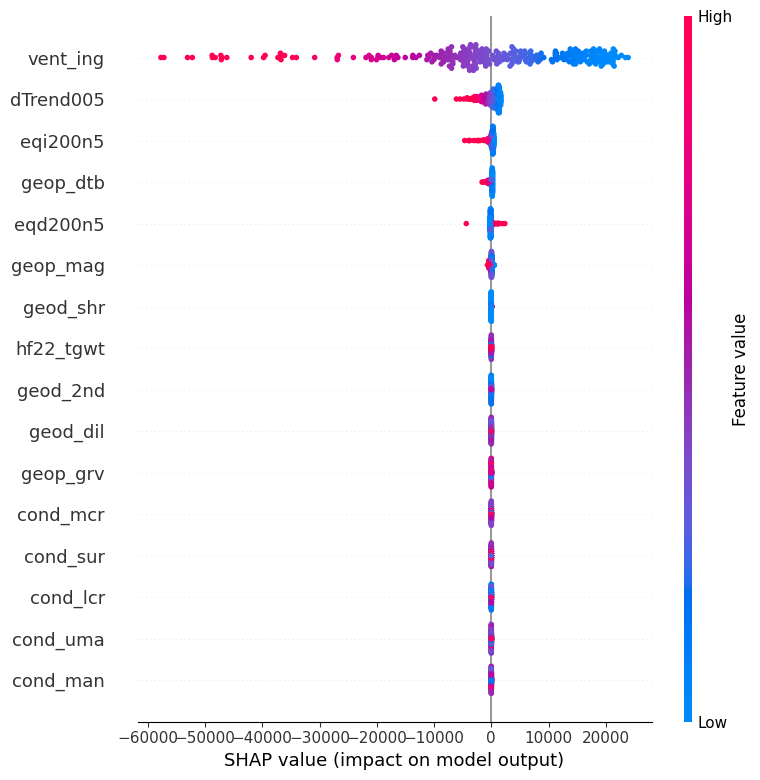
\includegraphics[width=0.5\textwidth]{SHAP.png}
\end{center}

\indent
The following graph shows the distribution of the predicted values. The model's predictions were fairly evenly distributed, with a slight bias towards the lower values. Because some label outliers were so high, the graph looks more skewed than it really should be after classifying.\\

\begin{center}
    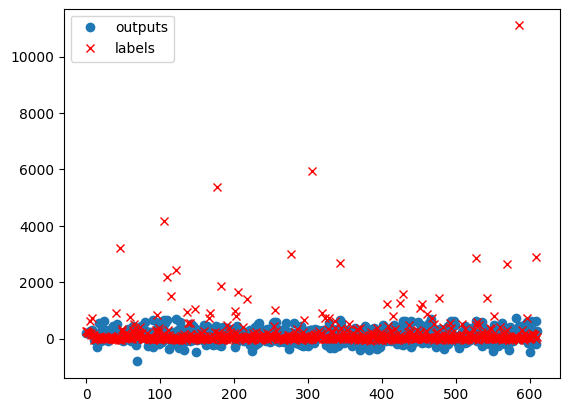
\includegraphics[width=0.5\textwidth]{output-label.png}
\end{center}

Finally, the following is a confusion matrix of each classification class. The model seemed to classify the lower values fairly well, but struggled with the higher values. Perhaps limiting the higher values to a smaller cap would improve the accuracy of the model. Because some of the higher values were so high, they skewed the data and made it more difficult to classify.\\

\begin{center}
    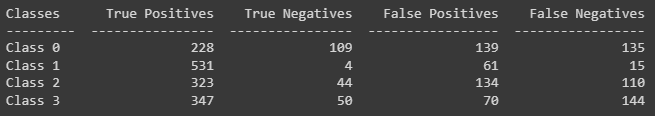
\includegraphics[width=0.5\textwidth]{confusion.png}
\end{center}

\section*{What I Learned}

This project provided an excellent opportunity to gain practical experience designing and training a nerual network on real data. The process of implementing most of the code from scratch and relying on documentation/other online resources allowed a deeper understanding of the process. The use of Optuna \cite{optuna_2019} was particularly valuable and provided a great introduction to hyperparameter optimization.\\
\indent
Additionally, this project served as as great practice for improving both EDA and general management skills, including data wrangling and data manipulation such as graphing and modifying data to gain insights on their behavior. Resources such as the PyTorch YouTube channel and online tutorials such as those referenced in the bibliography were invaluable in developing a strong understanding of the basics of neural networks and PyTorch.\\


\bibliographystyle{IEEEtran}
\bibliography{bibliography}

\end{document}